\chapter{Rocket Life Cycle}
\label{sec:rocketlifecycle}

This section is intended to give a high-level overview of the general process of engineering a rocket from scratch, regardless of the percentage of commercial off-the-shelf components used. The rocket life cycle begins once the team has committed to engineering a rocket for some purpose.

\section{Mission Planning}
\textbf{Evaluate goals}: SSI wide, rockets team wide, IREC team wide, subsystem. These should help form the guiding principles for what actually matters.\\

\textbf{Map out the external specifications for the rocket} (i.e. IREC rules and requirements). Keep those handy since it can be easy to forget about them after this phase of the life cycle. \\

\textbf{Identify key challenges} among all the requirements set on the team and the rocket. Try to use some team effort to begin to address mitigation strategies. This should be done throughout the process. \\

\textbf{Talk to other IREC teams} about past experiences. Identify teams you would like to emulate and stand on the shoulders of giants. In the past we've talked to: 
\begin{itemize}
\item Cal Poly
\item MIT
\item Oregon State University 
\end{itemize}
Here are some sample questions you can ask:
\begin{itemize}
\item What was your budget?
\item What did your timeline look like?
\item What was your biggest struggle?
\end{itemize}

\textbf{Optimize strategy for maximum points} within IREC. Look at the point spread and move on from there. Here is an excerpt of the 2016-17 IREC strategy:\\

\say{We also get 200 points for quality of design+build and amount of SRAD. The first big note we took from the category was that we cannot have tacked-on systems; everything needs to be planned out and well integrated. AKA if you think we are missing something, tell us ASAP so it doesn't become an afterthought. The second note is that a custom parachute is called out as being worth 25 points, so we will be attempting one (but not if it jeopardizes our altitude or recovery, which is worth far more.)}
\\

\textbf{Set safety factors}. This can be extremely difficult to do since there are often a lack of ways to do non-destructive tests. Here is a handy definition taken from our friends in Solar Car: \say{A factor of safety is a fudge factor that is actually a measurement of an engineer's confidence in their understanding of the design, manufacturing, and use case for an engineering project}.  \\

\textbf{Adhere to and set necessary loading conditions}. We have developed a set of loading conditions (but never enough). Similar to setting safety factors, this can be tough to accomplish without experience. They should look something like these:
\begin{itemize}
\item Recovery system is designed to separate at X m/s and all components must survive Y G's.
\item All components near charge must briefly survive Z temp.
\item All tubes and structural joints must withstand A mph wind shear occurring at a line across the middle of the rocket.
\end{itemize}
As Logan Herrera once said, \say{All loading conditions are supposed to actually match reality to B confidence level, and then we apply C safety factor}. \\

\textbf{Define subsystem}. Define purpose, upper bounds on size, and weight such that all goals, external specs, and strategy are satisfied. These definitions may be impossible to implement simultaneously; this is where the systems engineers work on compromise.  \\

\textbf{Project management begin}: set schedules, milestones, budgets, a communication plan, a task list, resource assessments and assignments, etc. This will be its own subsection, don't worry if this seems short.\\  

\textbf{Layout possible rocket configurations} based on your goals and IREC requirements. Pick one way of representing the rocket's length, weight, and space requirements and stick to it. For example, always have an updated Solidworks assembly which can spit out center of mass and locations of all components on the rocket worth modeling in simulation and integration. Have each subsystem 

\begin{figure}[h]
\centering
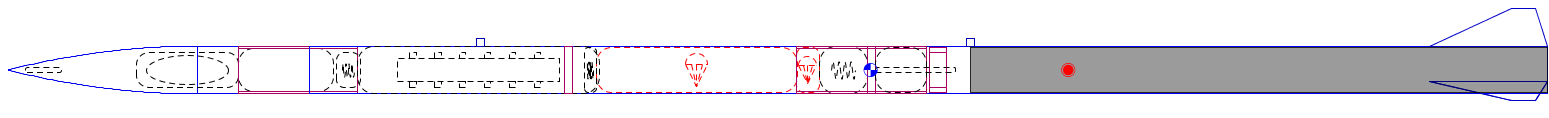
\includegraphics[width = 6in]{Figures/OR_layout.PNG}
\caption{OpenRocket layout}
\end{figure}

\textbf{Send configurations to simulations} for evaluation of feasibility and general order of magnitude (and a factor of 2 ;) analysis. \\

\textbf{Choose a rocket layout} after simulations come back. Add margin to both length and mass if you are aiming for an altitude-based goal. \\ 

\section{Prototyping}
This phase is pretty classic d.school. Begin work on concrete subsystem designs, exploring emph{different} ideas, so that we discover the best. We then choose our best guesses and present the rocket in a \textbf{Preliminary Design Review}. Throughout the process, each subsystem that can be non-destructively tested (or tested in pieces) is characterized as thoroughly as possible. 
\\

\section{Final Design Freeze}